\documentclass[conference]{IEEEtran}
\IEEEoverridecommandlockouts

\usepackage{cite}
\usepackage{amsmath,amssymb,amsfonts}
\usepackage{graphicx}
\usepackage{textcomp}
\usepackage{xcolor}
\usepackage{booktabs}
\usepackage{multirow}
\usepackage{url}
\usepackage{hyperref}

\begin{document}

\title{Closing the Offline-to-Live Gap in AI-Based SDN Intrusion Detection: Empirical Bottleneck Attribution and a Two-Stage Decoupled Defense}

\author{
\IEEEauthorblockN{Sijan Panday\IEEEauthorrefmark{1}, Research Partner\IEEEauthorrefmark{1}, and Manoj Shakya\IEEEauthorrefmark{1}}
\IEEEauthorblockA{\IEEEauthorrefmark{1}Department of Artificial Intelligence, DSAI Lab, Kathmandu University, Dhulikhel, Nepal}
}

\maketitle

\begin{abstract}
AI-based intrusion detection systems (IDS) for Software-Defined Networking (SDN) frequently report $>$99\% offline F1 scores on static flow datasets such as InSDN. However, offline classification accuracy does not reliably predict operational viability inside a live OpenFlow controller under volumetric or spoofed-header DDoS floods. Using an isolated, core-pinned Mininet, Open vSwitch 2.17, and \texttt{os-ken} OpenFlow 1.3 testbed across twelve logged experiments (\texttt{EXP-0001}--\texttt{EXP-0012}), we audit shortcut leakage in InSDN, calibrate the controller's synchronous compute ceiling, and decompose live per-\texttt{Packet-In} latency across base OpenFlow handling, feature extraction, synchronous \texttt{batch=1} inference, and cooperative \texttt{eventlet} loop starvation. Contrary to conventional assumptions, synchronous \texttt{batch=1} inference dispatch---not feature extraction---dominates per-event overhead: for a 65-feature Random Forest achieving 0.9998 offline F1, inference consumes 85.2\% of handler time (3.12\,ms of 3.66\,ms) versus 4.7\% (0.17\,ms) for feature extraction, collapsing benign new-TCP setup to 16.7\% at 250\,pps while flagging only 0.03\% of live spoofed floods due to single-packet observability blindness. Guided by these measurements, we design and ablate a Two-Stage Decoupled Defense (\texttt{A3}) combining an $O(1)$ Stage-1 port-rate gate and Selective Flow-Table Guard on the hot path with an out-of-process, core-pinned Stage-2 LightGBM classifier over 10 IP/port-agnostic 250\,ms OpenFlow window features. Across $N=5$ unseen seeds (75 trials), \texttt{A3} cuts controller CPU under 800\,pps UDP and TCP SYN floods from 97.5\%/96.8\% (synchronous LightGBM \texttt{A1}) to 5.1\%/4.4\% ($p=0.0119$), reduces peak switch flow-table occupancy 11.1$\times$--12.1$\times$ over unguarded asynchronous ML (\texttt{A2}, $p \le 0.0097$) with zero \texttt{TABLE\_FULL} refusals, and preserves 100.0\% legitimate completion under a 60\,conn/s benign TCP flash crowd where static rate limiting (\texttt{A4}) drops completion to 61.0\% ($p=0.0075$).
\end{abstract}

\begin{IEEEkeywords}
Software-Defined Networking, Intrusion Detection, DDoS Mitigation, Controller Bottleneck, Lightweight Machine Learning, OpenFlow.
\end{IEEEkeywords}

\section{Introduction}
Software-Defined Networking (SDN) centralizes network control via Southbound protocols such as OpenFlow 1.3, creating a natural vantage point for machine learning intrusion detection~\cite{janabi2024survey}. In reactive OpenFlow deployments, however, table-miss packets trigger \texttt{OFPPacketIn} events to the controller. Under spoofed-header DDoS floods, every packet spawns a distinct table miss, stressing both controller CPU and switch flow-table capacity~\cite{shin2013avantguard,wang2015floodguard}.

While numerous SDN-IDS studies report $>$99\% offline F1 on static \texttt{CICFlowMeter} benchmarks such as InSDN~\cite{elsayed2020insdn} and CIC-DDoS2019~\cite{sharafaldin2019cicddos}, offline evaluation omits three critical live systems constraints: (1)~\emph{observability mismatch}, because 65--80+ bidirectional flow statistics are unavailable at \texttt{Packet-In}~\#1 of a spoofed flood; (2)~\emph{synchronous control-plane blocking}, because Python controllers (\texttt{Ryu}/\texttt{os-ken}) execute handlers inside a single-threaded cooperative \texttt{eventlet} loop bound by the GIL; and (3)~\emph{benign flash-crowd collateral damage}, where naive rate limiters cannot separate legitimate connection surges from spoofed floods.

This paper addresses the central research question: \emph{How can we design and evaluate a lightweight AI-based SDN intrusion detection and mitigation system that maintains strong detection performance while minimizing live controller overhead under realistic traffic conditions?} Our main contributions are:
\begin{enumerate}
    \item \textbf{InSDN Leakage Audit \& Observability-Tier Benchmark:} We quantify feature duplication (36.4\%), identifier/port/TCP-window shortcuts, and \texttt{batch=1} vs.\ \texttt{batch=64} CPU latency across 4 SDN observability tiers and 5 model families (\texttt{EXP-0006}).
    \item \textbf{Empirical Compute-Budget Law \& Live Component Attribution:} Using core-pinned live execution (\texttt{EXP-0005}, \texttt{EXP-0007}), we locate a hard synchronous saturation cliff at 1.0--2.0\,ms per event at 250\,pps, prove that synchronous \texttt{batch=1} inference dominates over 65-feature extraction (85.2\% vs.\ 4.7\%), and document single-packet observability blindness (0.03\% live flood recall for a 99.98\% offline classifier).
    \item \textbf{Two-Stage Decoupled Defense \& Controlled $N=5$ Ablation:} We build and ablate five architectures (\texttt{A0}--\texttt{A4}) changing one mechanism at a time across 800\,pps UDP floods, 800\,pps TCP SYN floods, and 60\,conn/s benign TCP flash crowds (\texttt{EXP-0012}), validating every gain via Mann-Whitney U tests while explicitly reporting platform and workload threats to validity.
\end{enumerate}

\section{Related Work}
Existing SDN security literature splits sharply between systems-oriented control-plane defenses and offline-oriented AI detectors~\cite{janabi2024survey}.

\textbf{Control-Plane \& Flow-Table Protection:} AVANT-GUARD~\cite{shin2013avantguard} proxies TCP handshakes in the data plane to shield controllers from SYN floods, but cannot mitigate UDP floods and requires switch extensions. FloodGuard~\cite{wang2015floodguard} migrates table-miss bursts to a data-plane cache with rate-limited dispatch, and FlowRanger~\cite{wei2015flowranger} adds trust-based request prioritization; neither employs learned traffic discrimination to protect legitimate flash crowds. Flow-table exhaustion has been addressed via token-bucket bounding~\cite{xu2017tableoverflow}, adversarial timeout reconnaissance analysis~\cite{yu2021flowtable}, and low-rate overflow detectors such as FTMaster~\cite{tang2023ftmaster} and FloRa~\cite{mudgal2024flora}. None decompose live ML feature-extraction vs.\ inference latency inside the controller.

\textbf{AI-Based SDN-IDS \& Dataset Pitfalls:} Benchmark datasets such as InSDN~\cite{elsayed2020insdn} and CIC-DDoS2019~\cite{sharafaldin2019cicddos} rely on post-hoc \texttt{CICFlowMeter} extraction, which independent audits~\cite{engelen2021troubleshooting,liu2022errorprevalence,lanvin2023errors} show introduces flow-splitting bugs and testbed shortcuts. Recent GNN detectors~\cite{dadhania2024gnn} remain strictly offline. LUCID~\cite{doriguzzi2020lucid} achieves lightweight CNN DDoS classification on fixed packet windows, but profiles standalone offline replay outside an OpenFlow event loop. Two-stage entropy-plus-ML schemes~\cite{liu2022entropydl,hassan2024entropyml} evaluate average detection times in Mininet without decomposing tail latency (\texttt{p95}/\texttt{p99}), cooperative loop lag, flow-table refusals, or benign flash-crowd false blocking. QoSentry~\cite{khozam2025qosentry} highlights live benign QoS preservation via reinforcement learning, motivating our joint evaluation of controller overhead, flow-table occupancy, and benign new-flow QoS.

\section{Testbed, Telemetry, and Proposed Architecture}

\subsection{Core-Pinned Mininet/OVS Testbed \& Honest Instrumentation}
All live runs execute inside an isolated Ubuntu 22.04 Docker container (\texttt{ku-dsai-sdn:0.2}) running Mininet~2.3.0, Open vSwitch~2.17.12, and \texttt{os-ken}~2.11.0 (OpenFlow~1.3) on an AMD Ryzen 7 7840HS host (8C/16T, 15.19\,GB RAM). Because the host WSL2 kernel (\texttt{5.15.153.1-microsoft-standard-WSL2}) disables \texttt{CONFIG\_OPENVSWITCH} and \texttt{sch\_htb}/\texttt{sch\_netem}, OVS operates in userspace \texttt{netdev} mode with \texttt{ethtool} \texttt{veth} checksum/TSO/GSO offload disabled to prevent AF\_PACKET TCP drops. Strict \texttt{taskset} core pinning isolates \texttt{os-ken} (Core~0), traffic generators (Core~1), \texttt{ovs-vswitchd} (Cores~2--7), and the asynchronous Stage-2 worker (Core~8).

We deploy a 2-switch linear topology (\texttt{s1}--\texttt{s2}, \texttt{failMode=secure}) linking benign client \texttt{h\_benign} (\texttt{10.0.0.1}, \texttt{s1:p1}) and attacker \texttt{h\_attacker} (\texttt{10.0.0.2}, \texttt{s1:p2}) to victim \texttt{h\_server} (\texttt{10.0.0.3}, \texttt{s2:p2}). Both switches configure explicit software flow-table capacity (\texttt{flow\_limit=4096}, \texttt{overflow\_policy=refuse}), reported strictly as a \emph{software flow-table capacity proxy} rather than hardware TCAM. Between every trial, forwarding rules (\texttt{cookie=0x10}) and drop rules (\texttt{cookie=0x20}) are flushed after controller \texttt{Packet-In} quiescence with a hard zero-dynamic-flow assertion.

Every trial simultaneously measures (i)~controller \texttt{p50/p95/p99} handler latency (\texttt{perf\_counter\_ns}), (ii)~50\,ms \texttt{eventlet} heartbeat loop lag, (iii)~independent \texttt{os-ken}, worker, and \texttt{ovs-vswitchd} CPU/RSS, (iv)~\texttt{s1} flow-table occupancy and \texttt{TABLE\_FULL} counts, and (v)~three benign QoS probes: cached 20\,Mbps UDP \texttt{iperf3}, ICMP RTT, and a control-plane-sensitive \emph{new-TCP handshake probe} (2\,Hz under floods, 60\,Hz under flash crowds, 2.0\,s timeout).

\subsection{Two-Stage Decoupled Defense (\texttt{A3}) & Ablation Matrix}
Guided by our Phase~4 bottleneck diagnosis, \texttt{A3\_TwoStage\_Gate\_Decoupled\_TableGuard} separates fast-path control from ML inference:
\begin{itemize}
    \item \textbf{O(1) Windowed Telemetry:} \texttt{\_packet\_in\_handler} performs zero ML, updating 250\,ms per-\texttt{(dpid, in\_port)} rolling counters for 10 strictly IP/port-value-agnostic features: \texttt{packet\_in\_rate\_pps}, \texttt{unique\_src\_ip\_ratio}, \texttt{src\_ip\_entropy\_norm}, \texttt{unique\_src\_port\_ratio}, \texttt{dst\_ip\_concentration}, \texttt{udp\_ratio}, \texttt{tcp\_syn\_only\_ratio}, \texttt{tcp\_ack\_or\_est\_ratio}, \texttt{pkt\_len\_mean}, and \texttt{pkt\_len\_std}.
    \item \textbf{Stage-1 O(1) Gatekeeper \& Selective Flow-Table Guard:} Ports below 30\,pps incur zero Stage-2 IPC. Once an edge port crosses 30\,pps, it enters watch mode: the Selective Flow-Table Guard forwards via \texttt{OFPPacketOut} without installing unverified per-flow \texttt{OFPFlowMod} entries during the classification window, bounding switch flow-table growth while leaving unaffected ports untouched.
    \item \textbf{Stage-2 Core-8 Async ML Worker:} Suspicious 250\,ms feature vectors are dispatched non-blockingly over a direct \texttt{multiprocessing.Pipe} (avoiding \texttt{multiprocessing.Queue} feeder-thread conflicts with \texttt{eventlet}) to a LightGBM classifier pinned to Core~8. On positive detection ($P \ge 0.5$), the controller asynchronously installs a targeted priority-100 drop rule (\texttt{cookie=0x20}, \texttt{hard\_timeout=5\,s}, matching \texttt{(in\_port, ipv4\_dst, ip\_proto)}) on \texttt{s1}.
\end{itemize}

To isolate each mechanism cleanly, we ablate five architectures one variable at a time: \textbf{\texttt{A0}} (no-AI baseline), \textbf{\texttt{A1}} (synchronous per-\texttt{Packet-In} \texttt{T1a} LightGBM), \textbf{\texttt{A2}} (decoupled Core-8 windowed LightGBM + drop rules, running every 250\,ms without Stage-1 gating or table guard), \textbf{\texttt{A3}} (full proposed architecture), and \textbf{\texttt{A4}} (non-ML static rate threshold $\ge 30$\,pps installing immediate drops).

\section{Empirical Bottleneck Diagnosis (\texttt{EXP-0002}--\texttt{EXP-0008})}

\subsection{Baseline A Saturation \& Compute-Budget Cliff}
In \texttt{EXP-0002} (no AI, 0--1,500\,pps spoof sweep), \texttt{os-ken} saturated at 2,135\,Packet-In/s (96.98\% CPU), inflating loop lag 7.2$\times$ (0.97$\to$7.01\,ms) and dropping benign new-TCP survival to 37.5\% (2,165\,ms p95 at 1,000\,pps), while already-cached 20\,Mbps \texttt{iperf3} flows maintained 0.0\% loss---demonstrating why long-lived throughput probes miss control-plane collapse.

In \texttt{EXP-0005} ($N=3$ seeds, Core-0 pinned at 250\,pps $\approx 475$\,Packet-In/s), injecting synthetic synchronous work $t_{\text{AI}} \in [0, 4]$\,ms confirmed the single-core queueing ceiling $\mu_{\max}(t_{\text{AI}}) \approx 1000 / (t_{\text{base}} + t_{\text{AI}})$ ($t_{\text{base}} \approx 0.53$--0.63\,ms). As shown in Fig.~\ref{fig:exp0005}, crossing from 1.0\,ms (78.9\% CPU, 100\% TCP OK, 48.9\,ms p95) to 2.0\,ms triggers a steep cliff: 97.4\% CPU, 31.91\,ms loop lag (31$\times$), and 47.6\% TCP survival (1,293.7\,ms p95), worsening to 16.7\% survival at 4.0\,ms.

\begin{figure}[t]
\centering
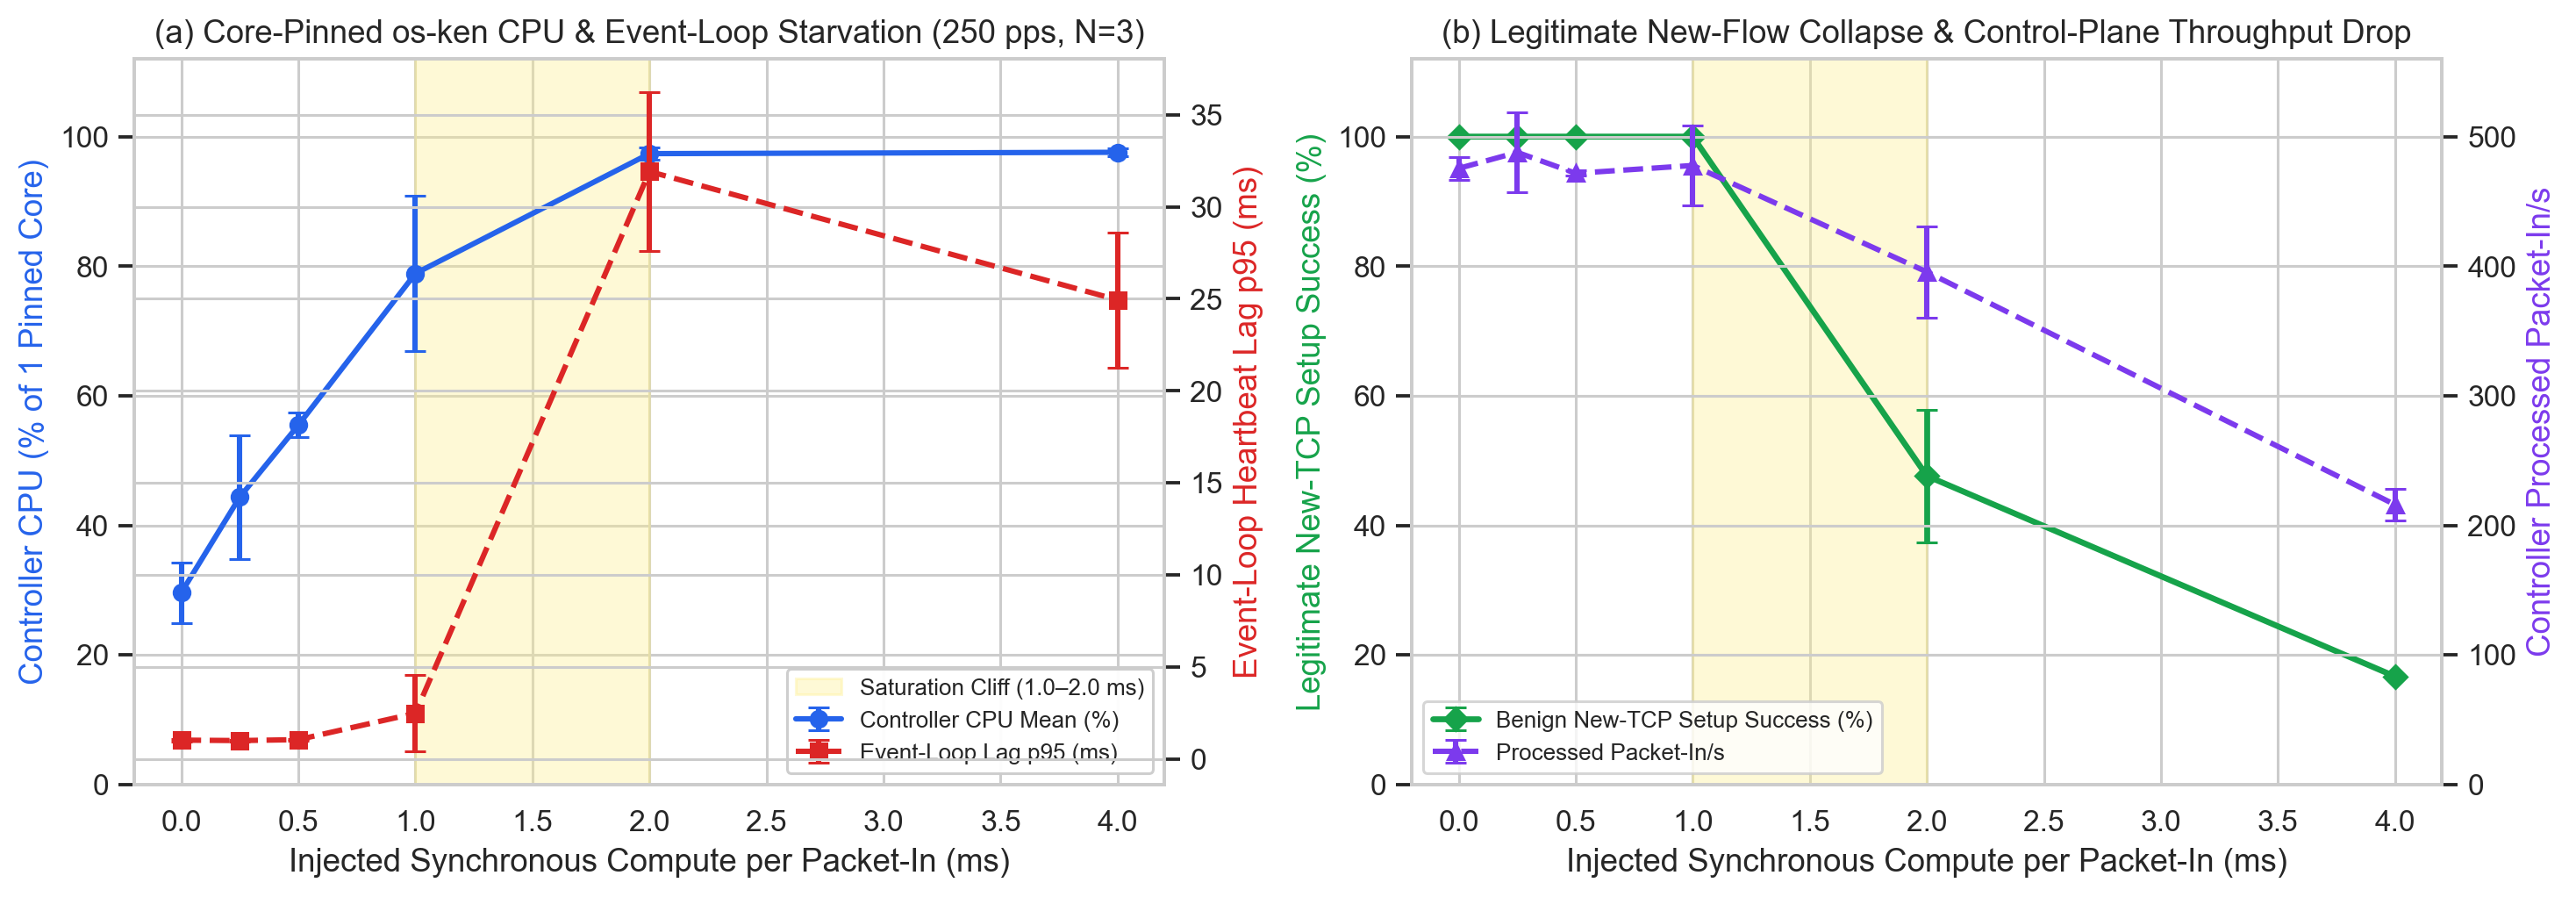
\includegraphics[width=\columnwidth]{../figures/fig02_exp0005_compute_budget_cliff.png}
\caption{Core-pinned synchronous compute-budget cliff (\texttt{EXP-0005}, 250\,pps spoof, $N=3$ seeds, mean $\pm$ 95\% CI). Exceeding 1.0--1.5\,ms per \texttt{Packet-In} saturates Core~0 and collapses benign new-TCP setup.}
\label{fig:exp0005}
\end{figure}

\subsection{InSDN Leakage Audit \& Offline Tier Trade-offs (\texttt{EXP-0006})}
Auditing raw InSDN (343,889 rows, 84 columns; SHA-256 verified) revealed 86.44\% of attacks use attack-only \texttt{Src IP}s, 12 columns have zero variance, and stripping identifiers exposes 125,252 feature-only duplicates (36.42\%, leaving 184,746 unique flows; Fig.~\ref{fig:exp0001}). Re-adding \texttt{Dst Port} inflated \texttt{T1a} LightGBM from 0.9661 F1 (4.37\% FPR) to 0.9979 F1 (0.12\% FPR). Similarly, the jump from \texttt{T1b} (0.9785 F1) to \texttt{T2} (0.9999 F1) was driven by \texttt{Init Bwd Win Byts} (importance 404), an OS TCP window-size fingerprint. Benchmarking single-threaded latency (\texttt{n\_jobs=1}, Fig.~\ref{fig:exp0006}) showed that \texttt{batch=1} dispatch latency is nearly invariant to feature count (LightGBM 0.52--0.59\,ms p50; Random Forest 5.50--7.01\,ms p50, violating the 1.0\,ms ceiling across all tiers), whereas micro-batching (\texttt{batch=64}) yielded 32.0$\times$--63.0$\times$ amortized speedups (0.003--0.114\,ms/flow).

\begin{figure}[t]
\centering
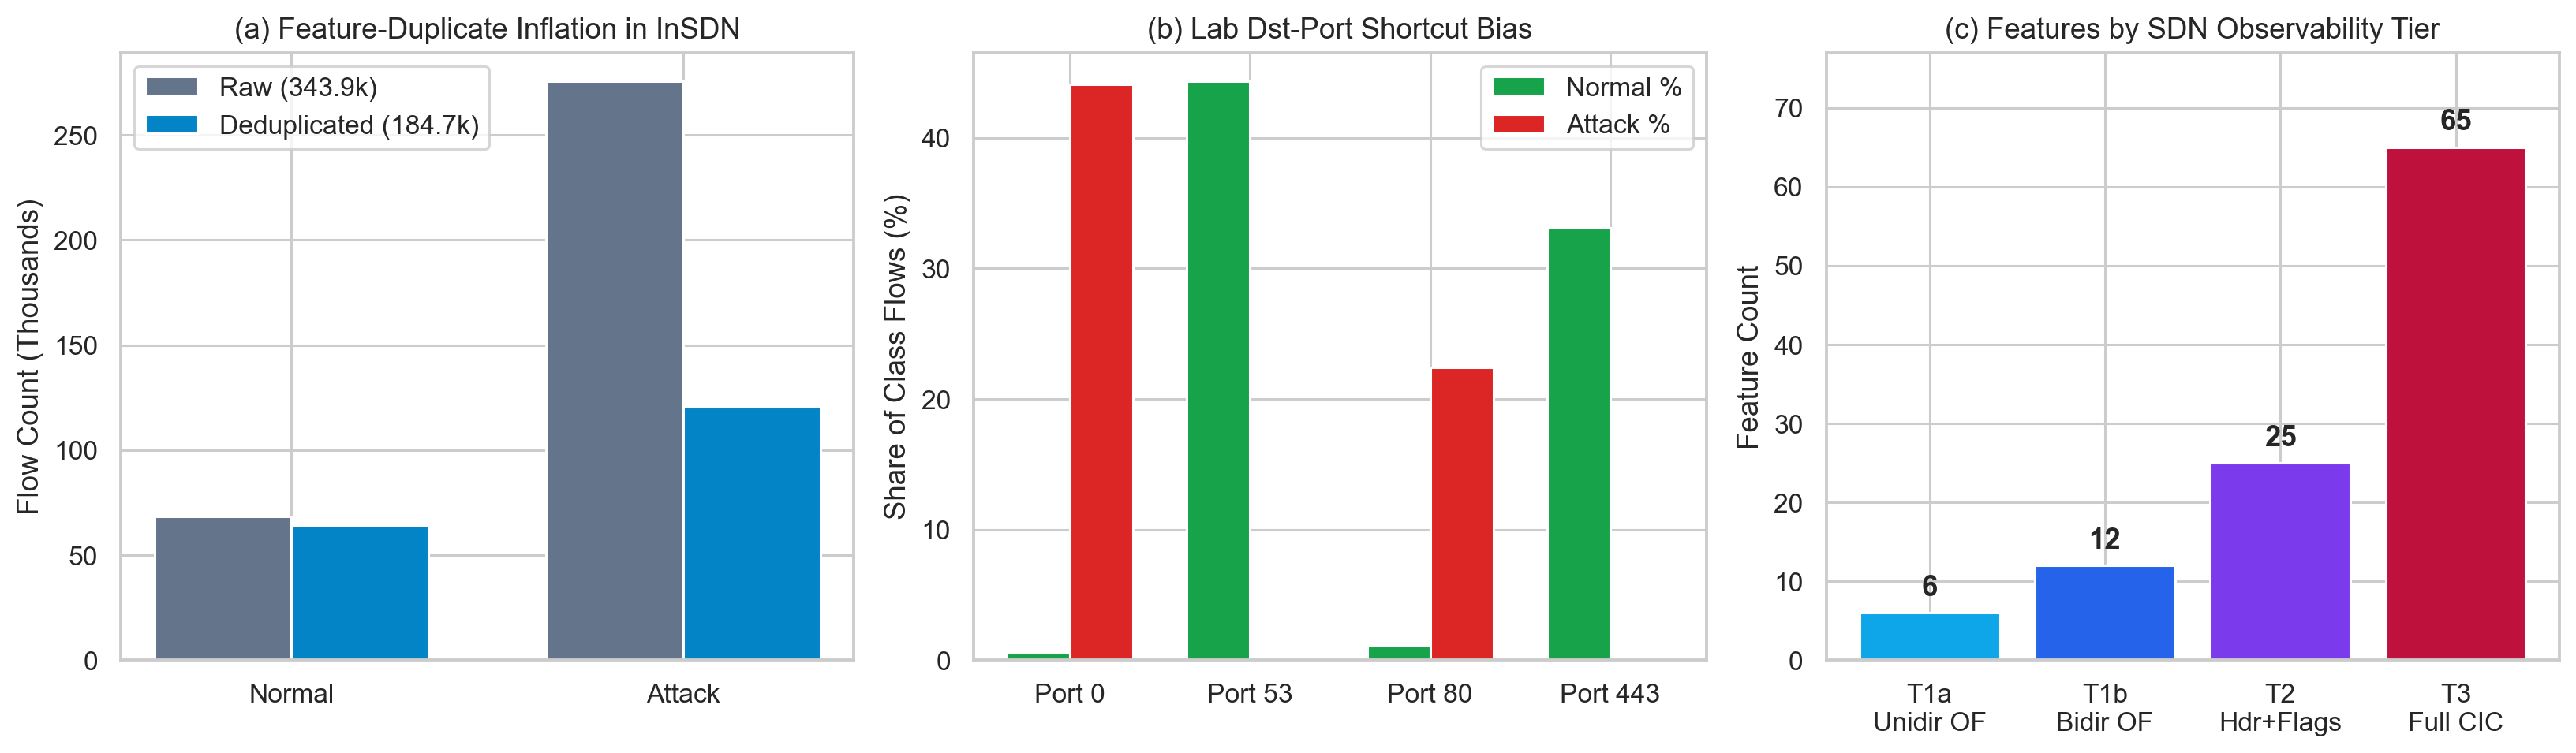
\includegraphics[width=\columnwidth]{../figures/fig01_insdn_leakage_and_tiers.png}
\caption{InSDN leakage audit (\texttt{EXP-0006}): 36.4\% feature-only duplication, IP/port shortcut separation, and observability-tier performance jump.}
\label{fig:exp0001}
\end{figure}

\begin{figure}[t]
\centering
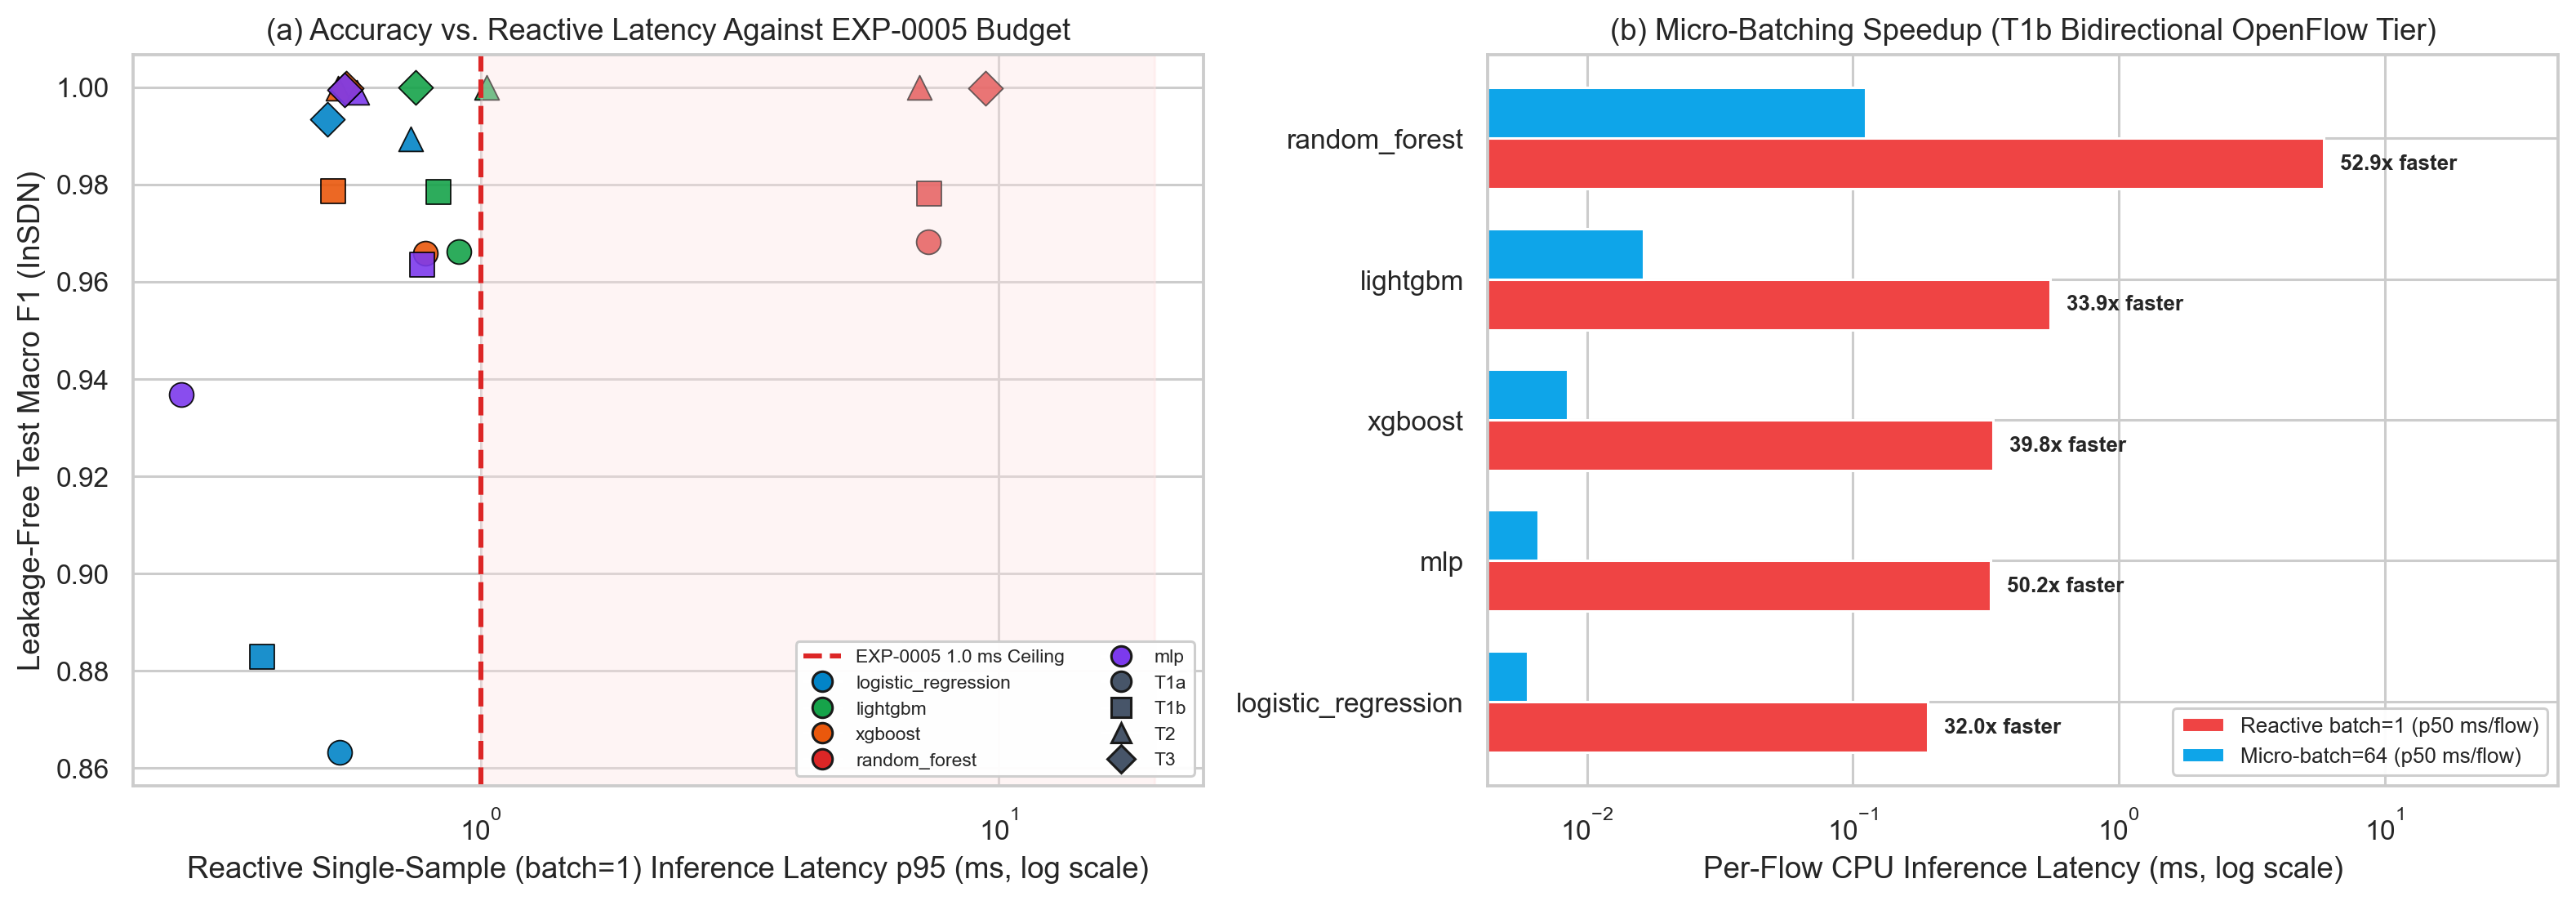
\includegraphics[width=\columnwidth]{../figures/fig03_exp0006_pareto_f1_vs_latency.png}
\caption{Offline Macro F1 vs.\ single-thread \texttt{batch=1} p95 latency (\texttt{EXP-0006}) compared against \texttt{EXP-0005}'s 1.0\,ms synchronous controller budget.}
\label{fig:exp0006}
\end{figure}

\subsection{Live Component Attribution \& Blindness (\texttt{EXP-0007})}
Table~\ref{tab:exp0007} and Fig.~\ref{fig:exp0007} present 24 core-pinned live trials ($N=3$ seeds $\times$ 8 pipelines at 250\,pps). Three findings directly shape our defense:
\begin{enumerate}
    \item \textbf{Inference Dominates Extraction (Refining Hypothesis H1):} On \texttt{Baseline\_C\_T3\_RF}, median handler time (3.66\,ms) splits into 0.35\,ms base OpenFlow (9.5\%), 0.17\,ms 65-feature extraction (4.7\%), and \textbf{3.12\,ms \texttt{batch=1} RF inference (85.2\%)}. On \texttt{T1a+LGBM}, inference (0.445\,ms) is 47$\times$ larger than extraction (0.009\,ms). Feature pruning alone cannot resolve synchronous dispatch saturation.
    \item \textbf{Offline-to-Live Collapse (Confirming H2):} Both \texttt{T1a+RF} and \texttt{T3+RF} (99.98\% offline F1) saturate Core~0 (98.1--98.3\% CPU), spike loop lag 24$\times$--29$\times$, and collapse benign new-TCP setup to 16.7--22.2\%.
    \item \textbf{Single-Packet Observability Blindness:} Because spoofed table-miss packets arrive as isolated 1-packet flows, the 99.98\% offline \texttt{T3+RF} classifier flagged only \textbf{1 of 2,684--3,225 live attack \texttt{Packet-In}s (0.03\%)} per trial.
\end{enumerate}

\begin{table}[t]
\centering
\caption{\texttt{EXP-0007} Live Component Attribution Inside Core-Pinned \texttt{os-ken} (250\,pps, $N=3$ Seeds)}
\label{tab:exp0007}
\resizebox{\columnwidth}{!}{%
\begin{tabular}{lccccccc}
\toprule
Pipeline & Off.\ F1 & Base (ms) & Extr.\ (ms) & Infer (ms) & Lag p95 & CPU (\%) & TCP OK \\
\midrule
\texttt{Baseline\_A\_NoAI} & --- & 0.329 & 0.000 & 0.000 & 1.02 & 30.15 & 100.0\% \\
\texttt{FeatsOnly\_T1a} & --- & 0.351 & 0.014 & 0.000 & 1.07 & 34.40 & 100.0\% \\
\texttt{FeatsOnly\_T3} & --- & 0.309 & 0.174 & 0.000 & 1.05 & 38.20 & 100.0\% \\
\texttt{B\_T1a\_LR} & 0.863 & 0.312 & 0.010 & 0.287 & 1.04 & 43.98 & 100.0\% \\
\texttt{B\_T1a\_LGBM} & 0.966 & 0.302 & 0.009 & 0.445 & 1.00 & 49.56 & 100.0\% \\
\texttt{B\_T1a\_XGB} & 0.966 & 0.310 & 0.010 & 0.405 & 1.04 & 49.51 & 100.0\% \\
\texttt{C\_T1a\_RF} & 0.969 & 0.348 & 0.009 & 3.173 & 24.56 & 98.07 & 22.2\% \\
\texttt{C\_T3\_RF} & 0.9998 & 0.346 & 0.172 & 3.118 & 29.46 & 98.33 & 16.7\% \\
\bottomrule
\end{tabular}%
}
\end{table}

\begin{figure}[t]
\centering
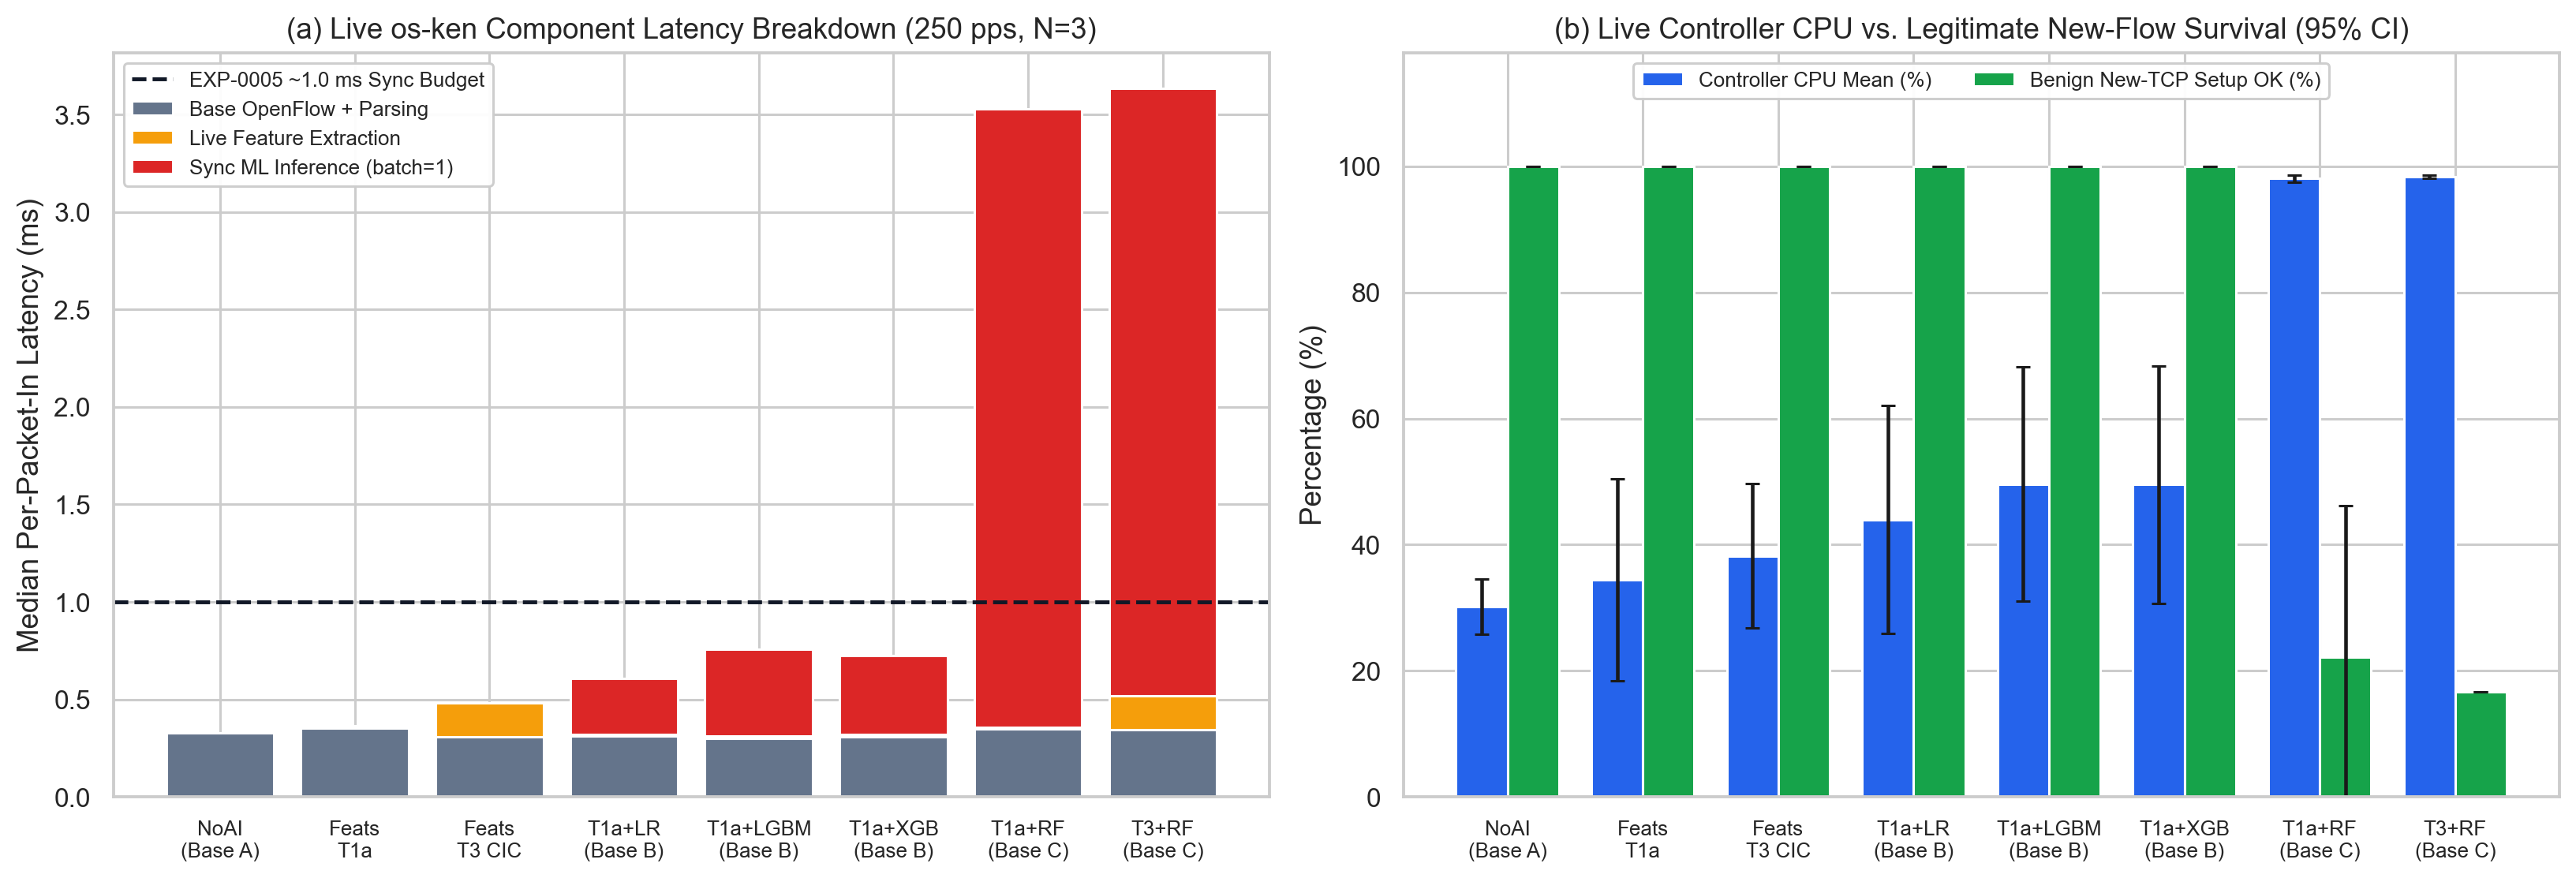
\includegraphics[width=\columnwidth]{../figures/fig04_exp0007_live_component_attribution.png}
\caption{Live component attribution (\texttt{EXP-0007}, $N=3$): \texttt{batch=1} inference dominates per-event latency (85.2\% on \texttt{T3+RF}) and triggers \texttt{eventlet} starvation.}
\label{fig:exp0007}
\end{figure}

\subsection{Multi-Regime Windowed Classifier (\texttt{EXP-0008})}
To overcome single-packet blindness, we collected 873 live 250\,ms per-port windows across 7 regimes (steady benign, 40/80\,Hz TCP flash crowds, 150/500\,pps variable-length spoofed UDP floods, and 150/500\,pps spoofed TCP SYN floods) over disjoint train seeds \texttt{[101,102]} and test seeds \texttt{[201,202]}. On held-out test seeds, \texttt{Static\_Rate\_Threshold} ($\ge 30$\,pps) achieved 0.6257 Macro F1 with \textbf{93.98\% flash-crowd FPR}, whereas our 10-feature \texttt{Stage2\_Window\_LightGBM} achieved 1.0000 Macro F1, 0.00\% flash-crowd FPR, and 100.0\% UDP/SYN recall.

\section{Phase 6 Controlled Ablation (\texttt{EXP-0012}, $N=5$ Seeds)}

Table~\ref{tab:exp0012} reports all 75 core-pinned trials across $N=5$ unseen seeds (\texttt{301}--\texttt{305}), 3 live scenarios, and 5 architectures; Fig.~\ref{fig:exp0012_floods} and Fig.~\ref{fig:exp0012_flash} visualize the flood and flash-crowd comparisons.

\begin{table*}[t]
\centering
\caption{\texttt{EXP-0012} Single-Variable Controlled Ablation ($N=5$ Unseen Seeds, 75/75 Trials, Mean $\pm$ 95\% CI)}
\label{tab:exp0012}
\begin{tabular}{llcccccccc}
\toprule
Scenario & Architecture & Ctrl CPU (\%) & Wrk CPU (\%) & Lag p95 (ms) & \texttt{s1} Occ.\ (\%) & \texttt{TABLE\_FULL} & IPC & False Mit. & Benign TCP OK / p95 (ms) \\
\midrule
\multirow{5}{*}{\texttt{spoof\_udp\_800pps}}
 & \texttt{A0} NoAI & $73.68 \pm 2.27$ & 0.24 & $1.51 \pm 0.22$ & $99.98 \pm 0.00$ & 8,052 & 0.0 & 0.0 & $100.0\% / 43.5$ \\
 & \texttt{A1} Sync LGBM & $97.52 \pm 0.20$ & 0.29 & $10.59 \pm 1.63$ & $99.98 \pm 0.00$ & 5,798 & 0.0 & 0.0 & $79.96\% / 1102.1$ \\
 & \texttt{A2} Decoupled & $5.64 \pm 0.48$ & 0.54 & $0.93 \pm 0.10$ & $16.32 \pm 1.29$ & 0 & 27.0 & 0.0 & $100.0\% / 12.4$ \\
 & \textbf{\texttt{A3} 2-Stage+Guard} & $\mathbf{5.13 \pm 0.71}$ & \textbf{0.34} & $\mathbf{0.86 \pm 0.08}$ & $\mathbf{1.47 \pm 0.08}$ & \textbf{0} & \textbf{4.2} & \textbf{0.0} & $\mathbf{100.0\% / 14.1}$ \\
 & \texttt{A4} Static Rate & $2.56 \pm 1.03$ & 0.30 & $0.87 \pm 0.10$ & $5.64 \pm 3.11$ & 0 & 0.0 & 0.0 & $100.0\% / 18.5$ \\
\midrule
\multirow{5}{*}{\texttt{spoof\_syn\_800pps}}
 & \texttt{A0} NoAI & $71.44 \pm 2.25$ & 0.30 & $1.42 \pm 0.24$ & $99.98 \pm 0.00$ & 8,052 & 0.0 & 0.0 & $100.0\% / 39.1$ \\
 & \texttt{A1} Sync LGBM & $96.84 \pm 0.84$ & 0.33 & $9.74 \pm 0.38$ & $99.98 \pm 0.00$ & 7,688 & 0.0 & 0.0 & $95.72\% / 1793.5$ \\
 & \texttt{A2} Decoupled & $5.82 \pm 0.63$ & 0.40 & $0.89 \pm 0.04$ & $17.38 \pm 2.12$ & 0 & 26.8 & 0.0 & $100.0\% / 11.3$ \\
 & \textbf{\texttt{A3} 2-Stage+Guard} & $\mathbf{4.42 \pm 0.52}$ & \textbf{0.28} & $\mathbf{0.89 \pm 0.08}$ & $\mathbf{1.44 \pm 0.00}$ & \textbf{0} & \textbf{4.2} & \textbf{0.0} & $\mathbf{100.0\% / 16.6}$ \\
 & \texttt{A4} Static Rate & $2.61 \pm 0.58$ & 0.30 & $0.82 \pm 0.12$ & $5.88 \pm 1.53$ & 0 & 0.0 & 0.0 & $100.0\% / 13.2$ \\
\midrule
\multirow{5}{*}{\texttt{benign\_flash\_60hz}}
 & \texttt{A0} NoAI & $23.52 \pm 0.54$ & 0.32 & $1.02 \pm 0.03$ & $30.82 \pm 1.00$ & 0 & 0.0 & 0.0 & $100.0\% / 15.5$ \\
 & \texttt{A1} Sync LGBM & $32.63 \pm 1.78$ & 0.34 & $1.07 \pm 0.03$ & $28.94 \pm 1.53$ & 0 & 0.0 & 0.0 & $100.0\% / 19.9$ \\
 & \texttt{A2} Decoupled & $23.01 \pm 0.84$ & 0.62 & $1.05 \pm 0.02$ & $28.88 \pm 0.97$ & 0 & 41.8 & 0.0 & $100.0\% / 15.5$ \\
 & \textbf{\texttt{A3} 2-Stage+Guard} & $\mathbf{23.50 \pm 0.60}$ & \textbf{0.64} & $\mathbf{1.05 \pm 0.03}$ & $\mathbf{28.92 \pm 0.17}$ & \textbf{0} & \textbf{40.0} & \textbf{0.0} & $\mathbf{100.0\% / 15.6}$ \\
 & \texttt{A4} Static Rate & $3.75 \pm 0.40$ & 0.36 & $1.16 \pm 0.20$ & $19.31 \pm 1.36$ & 0 & 0.0 & \textbf{4.0} & $\mathbf{60.97\% / 1070.7}$ \\
\bottomrule
\end{tabular}
\end{table*}

\begin{figure*}[t]
\centering
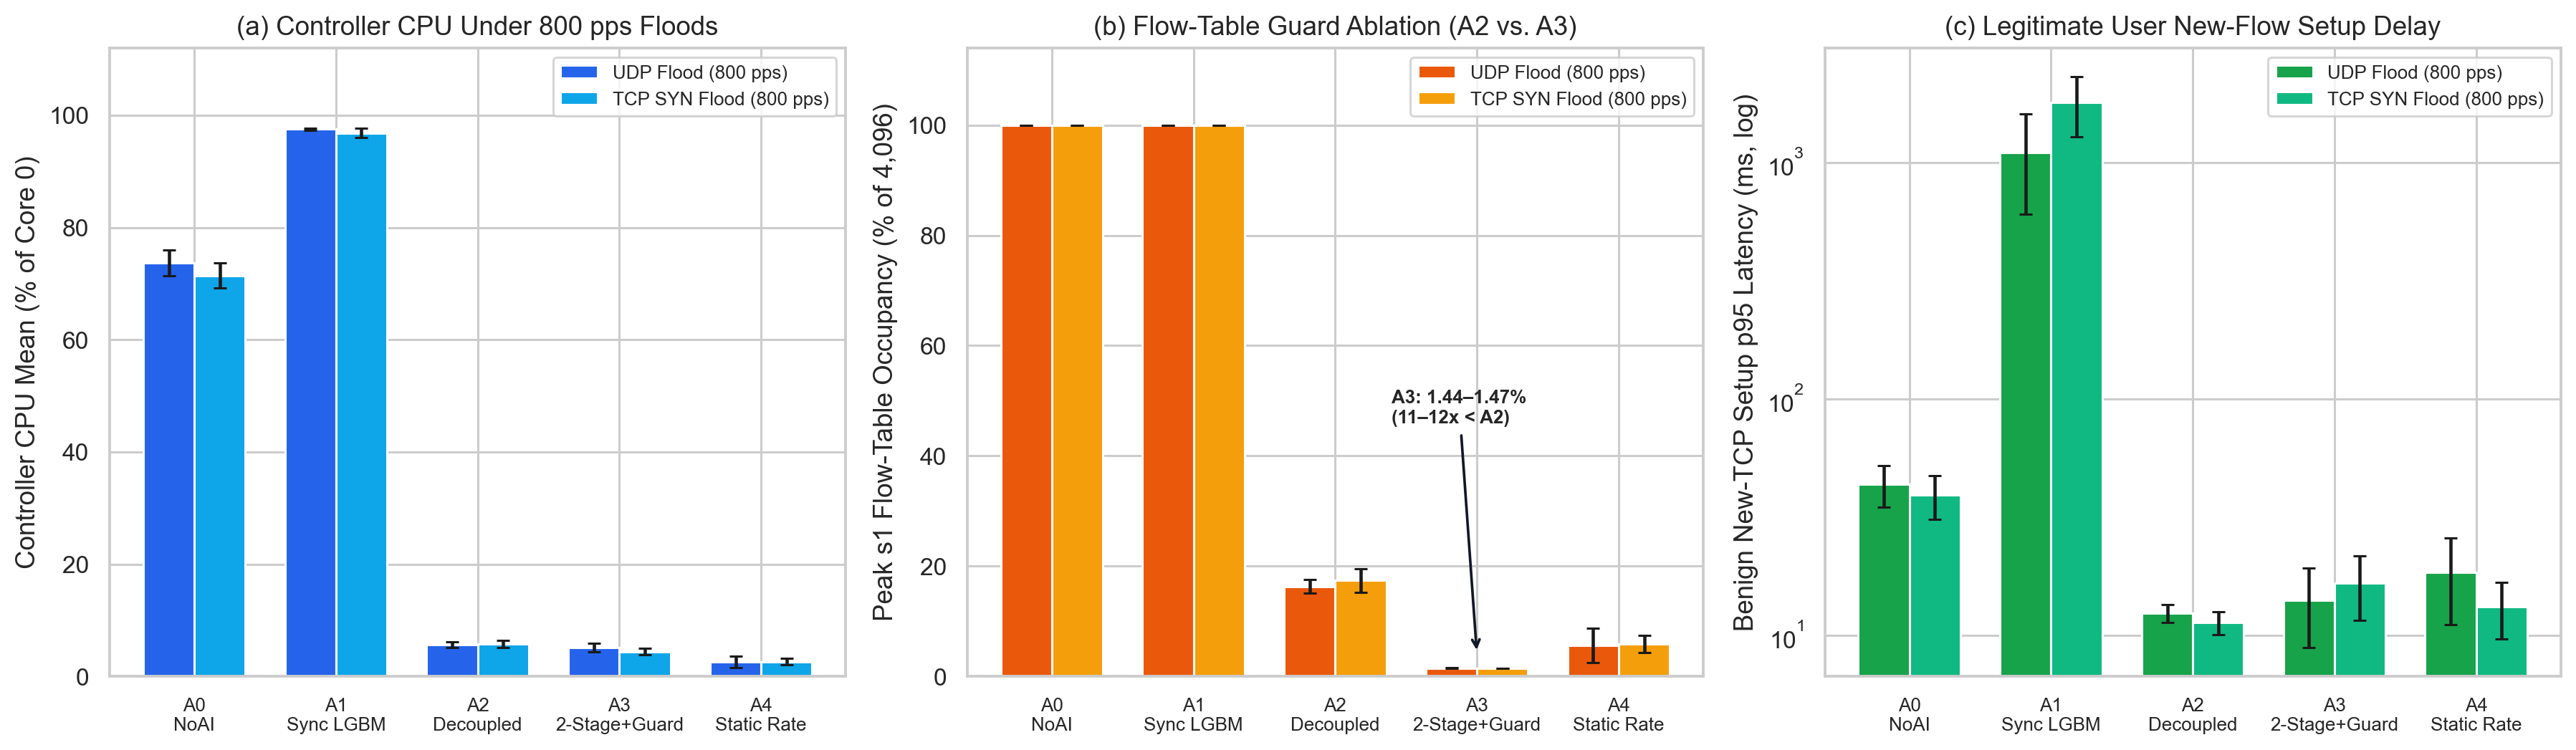
\includegraphics[width=\textwidth]{../figures/fig05_exp0012_ablation_floods.png}
\caption{\texttt{EXP-0012} flood ablation ($N=5$ seeds, mean $\pm$ 95\% CI): (a)~controller CPU collapse under \texttt{A1} vs.\ decoupling in \texttt{A2}/\texttt{A3}; (b)~11.1$\times$--12.1$\times$ flow-table occupancy reduction from \texttt{A3}'s Selective Flow-Table Guard; (c)~78$\times$--108$\times$ lower benign TCP setup p95 latency.}
\label{fig:exp0012_floods}
\end{figure*}

\begin{figure}[t]
\centering
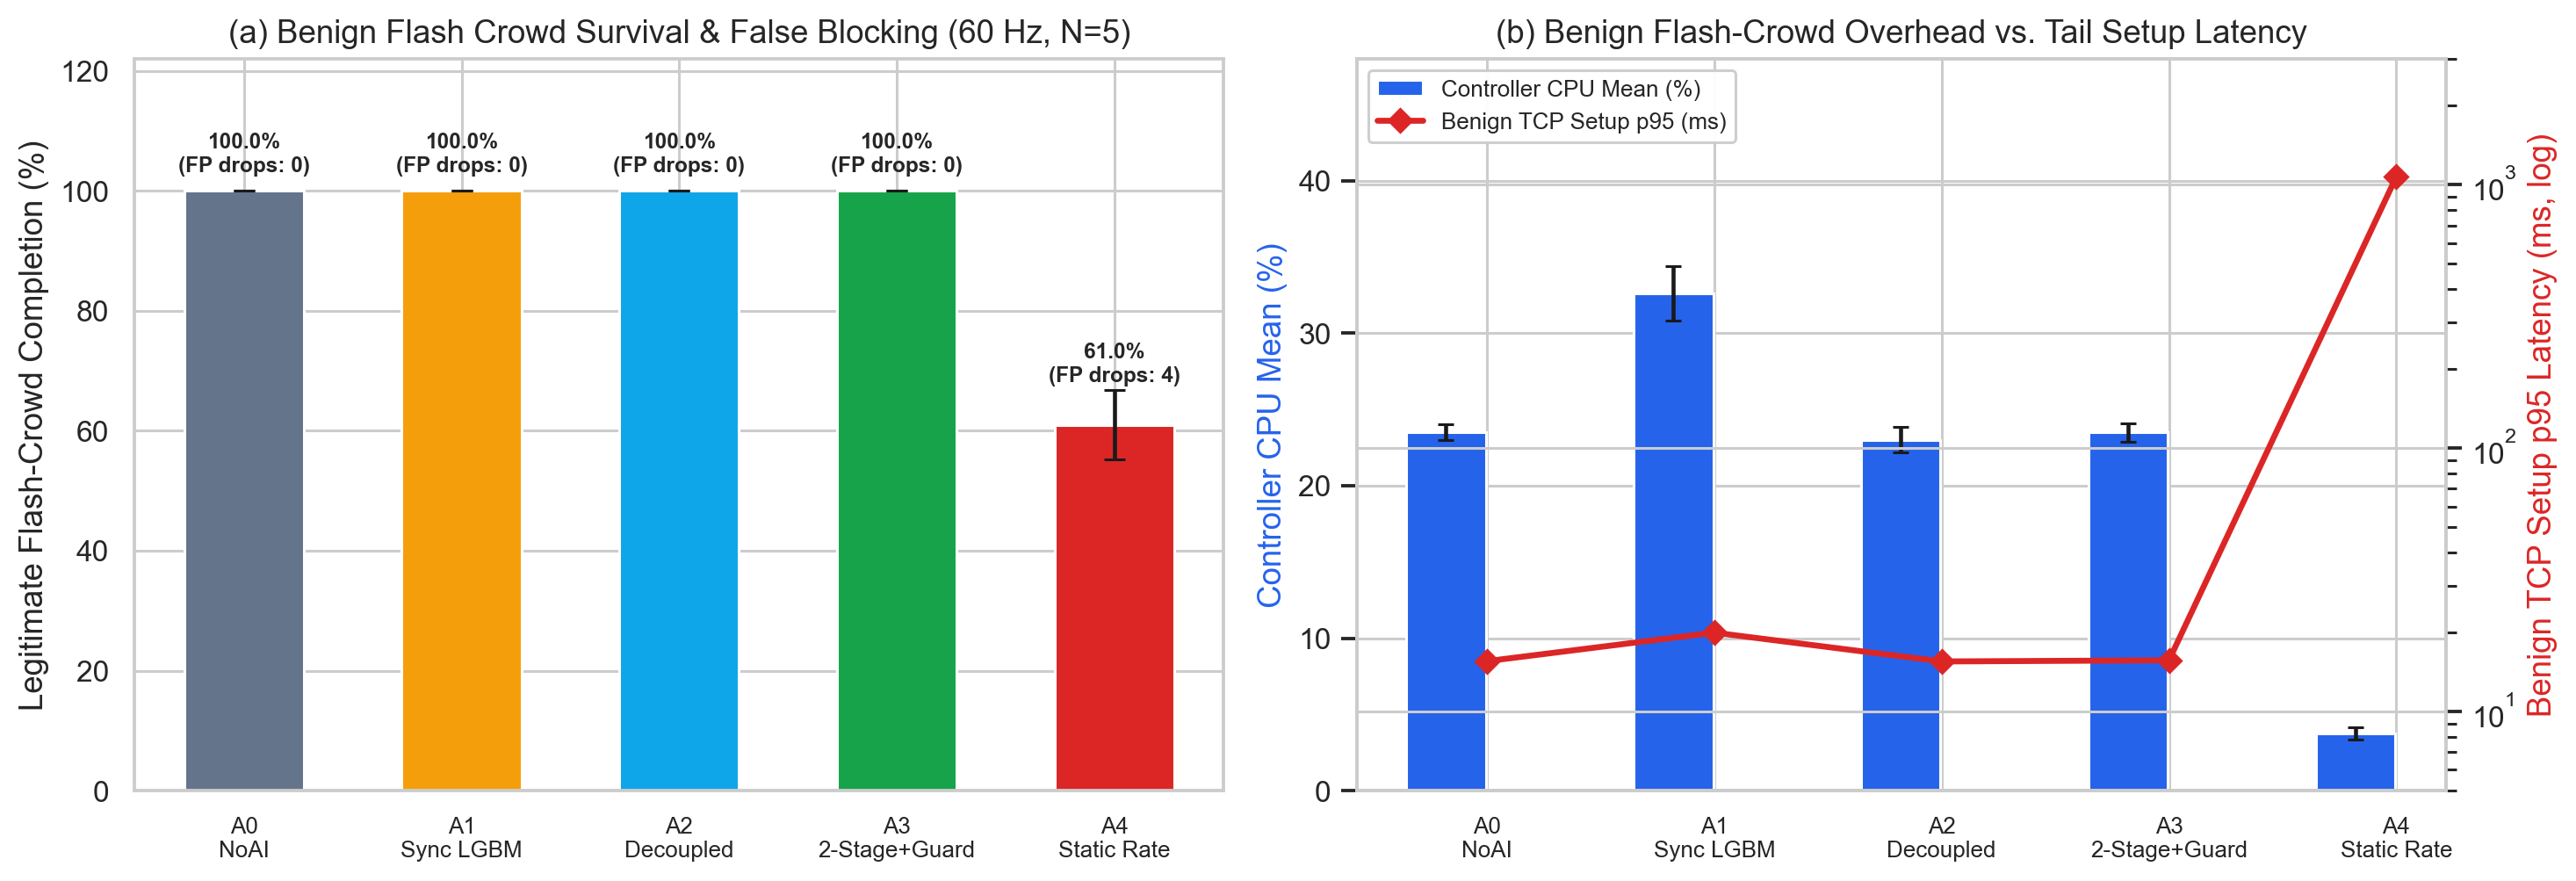
\includegraphics[width=\columnwidth]{../figures/fig06_exp0012_flash_crowd_vs_a4.png}
\caption{\texttt{EXP-0012} benign 60\,Hz TCP flash crowd ($N=5$): static rate limiting (\texttt{A4}) falsely blocks \texttt{h\_benign} 4 times/run, dropping completion to 61.0\% (1,071\,ms p95), whereas \texttt{A3} preserves 100.0\% completion at \texttt{A0} CPU parity.}
\label{fig:exp0012_flash}
\end{figure}

\textbf{Decoupling Effect (\texttt{A2}/\texttt{A3} vs.\ \texttt{A1}):} Under 800\,pps floods, even lightweight synchronous \texttt{T1a} LightGBM (\texttt{A1}) saturates Core~0 (97.5\% UDP / 96.8\% SYN), driving loop lag to 9.74--10.59\,ms and benign TCP setup p95 to 1,102--1,794\,ms. Decoupling (\texttt{A3}) reduces controller CPU to 5.13\% (UDP, $p=0.0119$) and 4.42\% (SYN, $p=0.0119$) with Stage-2 worker CPU $\le 0.34\%$, cuts loop lag to 0.86--0.89\,ms ($p=0.0079$), and restores 100.0\% benign TCP completion (UDP $p=0.0067$; on SYN, \texttt{A1}'s binary completion rate of 95.7\% yields $p=0.0668$, though \texttt{A1}'s p95 setup delay is 108$\times$ worse than \texttt{A3}'s 16.6\,ms).

\textbf{Stage-1 Gate \& Selective Flow-Table Guard (\texttt{A3} vs.\ \texttt{A2}):} During the 316--405\,ms detection-to-mitigation window, unguarded \texttt{A2} installs 632--798 spoofed rules (16.32--17.38\% of \texttt{s1}'s table) and submits 26.8--27.0 IPC windows. Adding the Stage-1 gate and Selective Flow-Table Guard (\texttt{A3}) slashes peak \texttt{s1} occupancy \textbf{11.1$\times$ on UDP (1.47\%, $p=0.0097$)} and \textbf{12.1$\times$ on SYN (1.44\%, $p=0.0075$)} with zero \texttt{TABLE\_FULL} errors and cuts IPC 6.4$\times$ (4.2 calls/run).

\textbf{Necessity of AI Under Flash Crowds (\texttt{A3} vs.\ \texttt{A4}):} Under 60\,conn/s benign TCP traffic, \texttt{A4} triggers 4.0 false port blocks per run ($p=0.0040$ vs.\ \texttt{A3}), collapsing legitimate completion to 60.97\% ($p=0.0075$) and inflating p95 delay 68.5$\times$ to 1,070.7\,ms. \texttt{A3} sustains 100.0\% completion, 0.0 false mitigations, 15.6\,ms p95, and 23.50\% CPU (matching \texttt{A0}'s 23.52\%, while \texttt{A1} wastes +9.1\% CPU at 32.63\%).

\section{Threats to Validity and Limitations}
\begin{enumerate}
    \item \textbf{WSL2 Userspace OVS vs.\ Native Linux Kernel:} Because WSL2 lacks \texttt{openvswitch.ko} and \texttt{tc} shapers, live experiments ran in userspace \texttt{netdev} mode without link-bandwidth shaping. While core pinning prevented OVS/controller CPU contention, absolute \texttt{Packet-In} ceilings must be replicated on a native Ubuntu Linux kernel with \texttt{TCLink} prior to journal submission.
    \item \textbf{Software Flow-Table Proxy:} Configured OVS \texttt{flow\_limit=4096} accurately tests bounded capacity enforcement, not physical ASIC TCAM lookup or rule-installation hardware limits.
    \item \textbf{Distributed Multi-IP Flash Crowds:} Our benign flash crowd originated from one client host (\texttt{10.0.0.1}), making source-IP entropy strongly discriminative in \texttt{EXP-0008}. Distributed multi-IP benign surges on shared aggregation ports will challenge source-cardinality features and require deeper bidirectional handshake features.
    \item \textbf{Topology Scale \& Stealthy Attacks:} Evaluating larger multi-switch topologies, low-rate flow-table overflow attacks~\cite{tang2023ftmaster,mudgal2024flora}, and adversarial evasion against windowed features remains future work.
\end{enumerate}

\section{Conclusion}
We demonstrated empirically that offline SDN-IDS accuracy fails to predict live control-plane survivability: inside a reactive OpenFlow controller, synchronous \texttt{batch=1} inference dispatch dominates per-event latency (85.2\% vs.\ 4.7\% for 65-feature extraction), crosses a hard queueing cliff at 1.0--2.0\,ms, and suffers 0.03\% live spoofed-flood recall due to single-packet observability blindness. Our Two-Stage Decoupled Defense (\texttt{A3}) resolves both control-plane saturation and switch flow-table exhaustion (5.1\%/4.4\% CPU, 1.44--1.47\% table occupancy, 0 \texttt{TABLE\_FULL}) while maintaining 100.0\% benign TCP flash-crowd survival where static rate limiting fails (61.0\%). All code, immutable manifests (\texttt{EXP-0001}--\texttt{EXP-0012}), notebooks, and raw metrics are archived for full reproducibility.

\bibliographystyle{IEEEtran}
\bibliography{references}

\end{document}
